\chapter{Discrete-Time Communication}
\label{chapter:DiscreteTimeComm}
\index{digital communication}

Most digital communication systems operate by converting digital data into continuous waveforms that can be conveyed through some physical medium to a receiver.
For example, digital communication through wires (e.g., Ethernet or USB) is based on moving electrons back and forth in the wire.
In contrast, underwater wireless communication uses acoustic transmission through the water.
While radio communication relies on the propagation of electromagnetic waves through air.

The process by which a string of bits is converted into a waveform suitable for transmission is known as \defn{digital communication}{modulation}.
The reverse operation, called \defn{digital communication}{demodulation}, is performed at the destination and involves extracting the information symbols from the received signal.
The mapping between the transmitted waveform and the received waveform is known as the \defn{digital communication}{channel}.

Precise models of the physical channel can be very complicated and many of the key ideas in digital communication do not depend on the exact details.
For this reason, one can model and design communication systems based a simplified model that separates the communication problem from the physical models.
In this chapter, we develop some basic concepts of digital communication using this simplified model.
The goal is to build some intuition about how things work without getting lost in the mathematical details.

\section{A Simple Channel Model}

\begin{figure}
\begin{center}
\scalebox{0.8}
{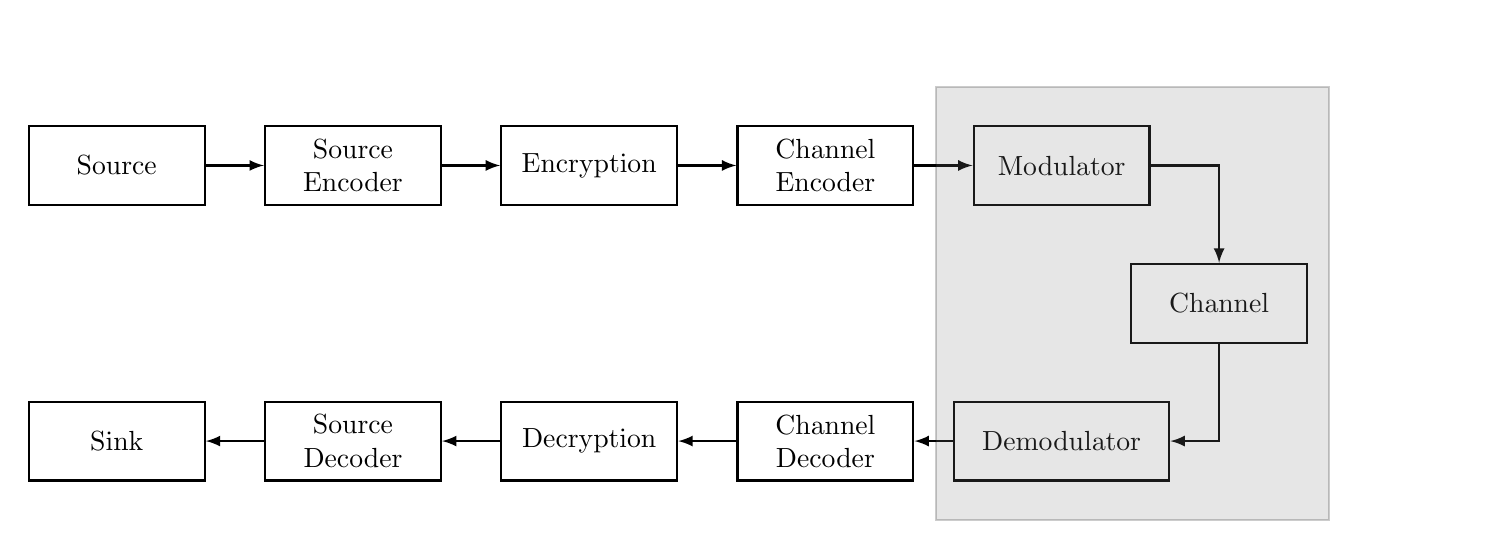
\begin{tikzpicture}[thick]
  \tikzstyle{every node}=[draw,text centered,text width=2cm,minimum height=1cm,shape=rectangle];
    \path (0,0) node (a) {Source}
          (0,1.25) node [draw=none] (aa) {}
          (3,0) node (b) {Source Encoder}
          (3,1.25) node [draw=none] (bb) {}
          (6,0) node (c) {Encryption}
          (6,1.25) node [draw=none] (cc) {}
          (9,0) node (d) {Channel Encoder}
          (9,1.25) node [draw=none] (dd) {}
          (12,0) node (e) {Modulator}
          (14,-1.75) node (f) {Channel}
          (16.25,-1.75) node [draw=none] (ff) {}
          (12,-3.5) node[text width=2.5cm] (g) {Demodulator}
          (9,-3.5) node (h) {Channel Decoder}
          (6,-3.5) node (i) {Decryption}
          (3,-3.5) node (j) {Source Decoder}
          (0,-3.5) node (k) {Sink};

    \draw[-latex] (a) -- (b);
    \draw[-latex] (b) -- (c);
    \draw[-latex] (c) -- (d);
    \draw[-latex] (d) -- (e);
    \draw[-latex] (e) -| (f);
    \draw[-latex] (f) |- (g);
    \draw[-latex] (g) -- (h);
    \draw[-latex] (h) -- (i);
    \draw[-latex] (i) -- (j);
    \draw[-latex] (j) -- (k);

    \filldraw[fill=gray,opacity=0.20] (10.4,1) rectangle (15.4,-4.5);
%    \draw (12.7,-5) node [draw=none,text width=10cm] (gg) {Discrete-Time Equivalent Channel};

\end{tikzpicture}}
\end{center}
\vspace{-4mm}
\caption{The block diagram of a digital communication system where the blocks comprising the discrete-time channel are shaded.}
\end{figure}

In this section, we introduce the \defn{digital communication}{discrete-time channel model} for digital communication systems.
We will see later that, for some communication systems, this model is exactly equivalent to the more complicated waveform model.
The first channel model we discuss is where the $n$th output of the channel, $Y_n$, is equal to the $n$th input to the channel, $x_n$, corrupted by an additive noise term $Z_n$ so that
\[ Y_n = x_n + Z_n. \]
For this model, it is typical to assume that the noise sequence $Z_1, Z_2, \ldots$ consists of independent identically distributed (i.i.d.) zero-mean Gaussian random variables with variance $\sigma^2$.
This implies that each $Y_n$ is a Gaussian random variable with mean $x_n$ and variance $\sigma^2$, so that
\[ f_{Y_n}(y_n) = \frac{1}{\sqrt{2\pi \sigma^2}} e^{-(y_n - x_n)^2 / (2\sigma^2)}.\]
This model is commonly referred to as discrete-time communication in \defn{digital communication}{additive white Gaussian noise} (AWGN) noise.

As an example, consider a system where the transmitter sets the voltage on end of a wire and the receiver measures the voltage on the other end of the wire.
It turns out that the thermal agitation of electrons causes voltage fluctuations known as Johnson noise.
So, the receiver ends up measuring the transmitted voltage corrupted by noise fluctuations.
In fact, Johnson noise is quite well approximated by AWGN.
So, the simple model described above already gives a relatively accurate picture of reality.

\section{A Simple Modulation Scheme}

Once a channel model has been defined, the next step is choosing how to transmit digital data through the channel.
A common approach is to choose a small set $\mathcal{U}$ of information symbols and represent each one by a distinct channel input in the set $\mathcal{X}$.
This is the discrete-time model of a scheme known as \defn{digital communication}{pulse-amplitude modulation} (PAM).
Let $u_n \in \mathcal{U}$ be the information symbol transmitted during the $n$th time interval and $x_n = M(u_n)$ be the $n$th input to the channel, where $M: \mathcal{U} \rightarrow \mathcal{X}$ is called the symbol mapping function.
For example, one can transmit binary information symbols by mapping ``0" to $+1$V and ``1" to $-1$V; mathematically, this is done by choosing $\mathcal{U}=\{0,1\}$, $\mathcal{X}=\{-1,1\}$, and $M(u) = 1-2u$.
This particular type of PAM is called \defn{digital communication}{binary phase-shift keying} (BPSK) or 2-PAM.

Suppose a BPSK signal is transmitted through our discrete-time AWGN channel model.
The detector must measure the voltage and decide whether a 0 or 1 one was transmitted.
A natural choice is to define a decoder function that associates positive voltages with 0 and negative voltages with 1.
Let $\hat{U}_n = D(Y_n)$ be the output of the detector function
\[ D(y) = \begin{cases} 0 & \text{if }y\geq0 \\ 1 & \text{if }y<0 \end{cases}. \]
This detector is optimal if 0's and 1's are transmitted with equal probability.

One of the main challenges in communication systems is providing reliable data transmission.
In this example, the noise variance $\sigma^2$ is proportional to the power of the thermal noise in the wire.
Notice that, if a 1 is transmitted, the detector described above will make an incorrect decision with probability
\[ \Pr \left( Y_n \geq 0 | x_n = 1 \right) = \Pr \left( Z_n \geq 1 \right) = \int_{1}^{\infty}  \frac{1}{\sqrt{2\pi \sigma^2}} e^{-y^2 / (2\sigma^2)} dy = Q\left( \frac{1}{\sigma} \right).\]
This probability can be reduced by increasing the transmitted voltage, which increases the power dissipated due to resistive losses, or by reducing the thermal noise.
For this reason, receivers used for large satellite dish receivers often use liquid nitrogen to cool the first-stage amplifier to reduce this thermal noise.
On the other hand, the maximum transmitted power is typically limited by physical constraints (e.g., the wire thickness) or FCC regulations.

\begin{figure}[t]
\begin{center}
\scalebox{0.75}
{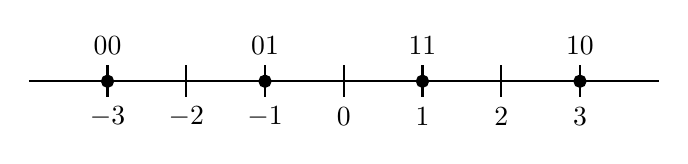
\begin{tikzpicture}[thick]

  \draw (-4,0) -- (4,0);

  \foreach \x in {-3,-2,...,3}
  {
    \draw (\x,-0.20) -- (\x,0.20);
    \draw (\x,-0.45) node {$\x$};
  }

  \foreach \x/\y in {-3/00,-1/01,1/11,3/10}
  {
    \draw (\x,+0.45) node {$\y$};
    \filldraw (\x,0) circle (2pt);
  }

\end{tikzpicture}}
\end{center}
\vspace{-6mm}
\caption{The symbol set $\mathcal{X}$ for 4-PAM with gray coded binary labels.}
\end{figure}

To send more information per channel use, one can use larger sets of PAM symbols.
For example, 4-PAM uses the 4 symbols $\mathcal{X}=\{ -3,-1,1,3 \}$ while 8-PAM uses the 8 symbols $\mathcal{X}=\{-7,-5,-3,-1,1,3,5,7\}$.
Notice that these two sets of symbols are centered around 0 to minimize the transmitted energy.

The mapping function $M(\cdot)$ determines the information symbol associated with each channel input value.
In general, sets of input values with $2^m$ elements are associated with binary strings.
There are still some choices to be made, however, because one can map the 4-PAM symbol set to binary strings in either the standard binary order $\{00,01,10,11\}$ or with a Gray code $\{00,01,11,10\}$.

For the 4-PAM symbol set with the mapping function $M(\cdot)$ that maps $\{00,01,10,11\}$ (in order) to $\{-3,-1,1,3\}$, the natural decision function is
\[ D(y) = \begin{cases}
00 & \text{if }y < -2 \\
01 & \text{if }-2 \leq y<0 \\
10 & \text{if }0 \leq y< 2 \\
11 & \text{if }y \geq 2
\end{cases}. \]

\section{Quadrature Amplitude Modulation}

In most communication systems, the baseband waveform is modulated onto a high-frequency carrier to enable better propagation.
This is because low-frequency signals often do not propagate well through physical media.
While this process will be discussed later in more detail, the following key detail affects the discrete-time model.
High frequency modulation allows two independent signals to be modulated onto the same carrier frequency; one onto the sine wave and the other onto the cosine wave.
This allows one to treat the transmitted value $x_n$ and received value $Y_n$ as points in 2-dimensional space.
The set $\mathcal{X}$ of possible transmitted points in 2-dimensional space in called the \defn{digital communication}{symbol constellation}.

\begin{figure}
\begin{center}
\scalebox{0.5}
{\begin{tikzpicture}[thick]

  \draw (-4,0) -- (4,0);
  \draw (0,-4) -- (0,4);

  \foreach \x in {-3,-2,...,3}
    \draw (\x,-0.20) -- (\x,0.20);

  \foreach \y in {-3,-2,...,3}
    \draw (-0.20,\y) -- (0.20,\y);

  \foreach \x in {-3,-1,1,3}
  \foreach \y in {-3,-1,1,3}
  {
    \filldraw (\x,\y) circle (2pt);
  }

\end{tikzpicture}}
\hspace{5mm}
\scalebox{0.5}
{\begin{tikzpicture}[thick]

  \draw (-4,0) -- (4,0);
  \draw (0,-4) -- (0,4);

  \foreach \x in {-3,3}
    \draw (\x,-0.20) -- (\x,0.20);

  \foreach \y in {-3,3}
    \draw (-0.20,\y) -- (0.20,\y);

  \foreach \x/\y in {3/0,2.12/2.12,0/3,-2.12/2.12,-3/0,-2.12/-2.12,0/-3,2.12/-2.12}
  {
    \filldraw (\x,\y) circle (2pt);
  }

\end{tikzpicture}}
\end{center}
\caption{The symbol constellations $\mathcal{X}$ for 16-QAM (left) and 8-PSK (right).}
\end{figure}

For mathematical convenience, points in these two-dimensional symbol constellations are represented by complex numbers.
The set of complex numbers is $\mathbb{C}$ and the constellation is a subset $\mathcal{X}\subset\mathbb{C}$.
Likewise, the transmitted symbol is $x_n \in \mathbb{C}$ and the received value is $Y_n \in \mathbb{C}$.
The noise term $Z_n$ now consists of two i.i.d. Gaussian random variables (one in each direction).
The probabilistic observation model is formed by treating the real and imaginary parts separately, and is given by
\begin{align*}
f_{Y^{(r)}_n,Y^{(i)}_n}(y^{(r)}_n,y^{(i)}_n) & =
\left( \frac{1}{\sqrt{2\pi \sigma^2}} e^{-\left(y^{(r)}_n - x^{(r)}_n\right)^2 / (2\sigma^2)} \right)
\left( \frac{1}{\sqrt{2\pi \sigma^2}} e^{-\left(y^{(i)}_n - x^{(i)}_n\right)^2 / (2\sigma^2)} \right) \\
& =  \frac{1}{2\pi \sigma^2} e^{-\left|y_n - x_n\right|^2 / (2\sigma^2)}.
\end{align*}
Therefore, the probability of receiving a $y_n$ value is simply a function of its Euclidean distance $\left| y_n - x_n \right|^2$ from the actual transmitted symbol.
This leads to a nice geometric characterization of the optimal decision regions for the detector.

The \defn{digital communication}{signal-to-noise ratio} (SNR) of a communication system is typically denoted by $E_s / N_0$ where $E_s$ is the average \textbf{energy per channel input symbol} and $N_0$ is the \defn{digital communication}{noise spectral density}.
For equiprobable signaling, one finds that
\[ E_s = \frac{1}{|\mathcal{X}|} \sum_{x\in \mathcal{X}} |x|^2. \]
The noise spectral density measures how much the AWGN is affects the channel and later we will see that $N_0 = 2 \sigma^2$ for our discrete-time model.

Constellations are typically defined by first choosing the set of channel input values $\mathcal{X}$, and then choosing the mapping function $M:\mathcal{U} \rightarrow \mathcal{X}$.
This second step is called \textbf{labeling} the constellation.
While the labeling does not affect the symbol error rate of the system, it generally does affect the bit error rate.
Therefore, one can optimize the mapping function for a particular application.

Constellations can be chosen and optimized for a variety of reasons.
Still, there are a few very common choices:
\begin{itemize}
\item $M$-ary PAM ($M$-PAM) is $M$ points equally spaced along a line or
\[ \mathcal{X} = \left\{ 2a-(M-1) \, \big| \, a \in \{0,1,\ldots,M-1\} \right\} \subset \mathbb{C}. \]

\item $M^2$-ary QAM ($M^2$-QAM) is an $M$ by $M$ square grid of points or
\[ \mathcal{X} = \left\{ \left(2a-(M-1)\right)+ \left(2b-(M-1)\right)i \, \big| \, a,b \in \{0,1,\ldots,M-1\} \right\} \subset \mathbb{C}. \]

\item $M$-ary PSK ($M$-PSK) is $M$ points equally spaced around a circle or
\[ \mathcal{X} = \left\{ e^{2\pi i k/M} \, \big| \, k \in \{0,1,\ldots,M-1\} \right\} \subset \mathbb{C}. \]
\end{itemize}

\begin{example}
The standard QAM constellation with 16 points (known as 16-QAM) is given by
\[ \mathcal{X} = \left\{ a+bi \, \big| \, a,b \in \{-3,-1,1,3\} \right\} \subset \mathbb{C}. \]
The average energy of this constellation is given by
\[ E_s = \frac{1}{16} \sum_{a,b\in \{-3,-1,1,3\}} (a^2 + b^2) = \frac{8}{16}  \sum_{a\in \{-3,-1,1,3\}} a^2 = 10.\]
\end{example}

\section{Optimal Symbol Detection}
\index{hypothesis testing}

In this section, we consider the problem of designing a symbol detector that minimizes the probability of error.
This is known as an \defn{digital communication}{optimal detection} problem and has an elegant solution that is related to the classical problem of \textbf{hypothesis testing} in statistics.

\subsection{Hypothesis Testing}

Sir Ronald Fisher, one of the founders of statistical decision theory, was at a tea party when Ms. Bristol mentioned that she preferred tea poured into milk over milk poured into tea.
Fisher commented that surely she could not tell the difference, but his colleague William Roach suggested that they design an experiment.
At that point, they prepared eight cups of tea: four milk-into-tea and four tea-into-milk.
The cups were presented in a random order and she correctly identified enough (all eight cups by some accounts) to prove her point.

Adding math to this requires that one defines carefully ``can tell the difference", but this is not a big problem because, for example, one can use the hypothesis $H_0=$``her success rate is more than three out of four".
There are more subtle issues, however, such as the meaning of passing the test.
While Ms. Bristol may do this by luck, this is also easy to analyze with calculations.
What is more problematic is understanding all the other hypotheses that can lead to the same observation.
For example, she may pass by cheating but still be unable to distinguish between the two drinks.
If this hypothesis is not explicitly considered, one can come to an incorrect conclusion.

For this reason, any scientific test of a hypothesis can only \emph{disprove} that hypothesis.
If Ms. Bristol cannot get 75\% correct in a larger test, then we can be reasonably confident that ``her ability to distinguish does not meet our threshold of three times out of four".
This is an example of a \defn{hypothesis testing}{null hypothesis} statistical test where the hypothesis can only disproven reliably.
Adding some math to this example shows that
\[ \Pr (\text{she identifies all cups correctly} | H_0 \text{ is false}) \leq (3/4)^8 \approx 0.10. \]
Therefore, the observation does not support the falsification of $H_0$.
Not much more can be concluded from this experiment.

\subsection{Multiple Hypothesis Testing}

Hypothesis testing in communication theory often has the luxury that one of the hypotheses must be true.
This leads to the more well-defined problem of \defn{hypothesis testing}{multiple hypothesis testing}.
Instead of testing a single hypothesis to see if it is false, one can compare multiple hypothesis to see which is most supported by the observation.

Let $H_0,H_1,\ldots,H_{m-1}$ be $m$ different hypotheses that affect a random observation $Y$.
The probability of a hypothesis before the observation, $\Pr(H_i)$, is called the \defn{hypothesis testing}{a priori probability}.
For each hypothesis, the connection with $Y$ is defined by the \defn{hypothesis testing}{observation probability} $\Pr (Y=y \, | \, H_i)$.

The goal is to choose a decision function $D(y)$ which, for any observation, minimizes the decision error probability.
Of course, this is equivalent to maximizing the probability that the decision is correct.
Notice that, if $Y=y$, then the probability that hypothesis $H_i$ is correct is given by its \defn{hypothesis testing}{a posteriori probability} $\Pr (H_i \, | \, Y=y )$.
Therefore, one finds that the optimal choice is the \defn{hypothesis testing}{maximum a posteriori} \textbf{probability} (MAP) decision rule 
\[ D(y) = \underset{i\in\{0,\ldots,m-1\}}{\mathrm{arg\,max}} \Pr( H_i \, |  \, Y=y). \]

In practice, these probabilities can be computed with Bayes' rule using only the a priori probabilities and observation probabilities.
This gives
\[ \Pr \left(H_i | Y=y \right) =
\frac{\Pr(H_i) \Pr (Y=y | H_i) }{\sum_{j=0}^{m-1} \Pr(H_j) \Pr (Y=y | H_j)}. \]
Since the denominator of this expression is the same for all $i$, the MAP rule can be simplified to
\[ D(y) = \underset{i\in\{0,\ldots,m-1\}}{\mathrm{arg\,max}} \Pr(H_i) \Pr (Y=y | H_i). \]

\begin{example}
Consider a system which transmits BPSK over an AWGN channel.
Let $H_0$ be the hypothesis that a zero (i.e., $+1$) was sent and $H_1$ be the hypothesis that a one (i.e., $-1$) was sent.
For binary hypothesis problems, the MAP decision rule can be written as
\[ \Pr (H_0) \Pr (Y=y | H_0) \underset{H_1}{\overset{H_0}{\gtrless}}  \Pr (H_0) \Pr (Y=y | H_0, \]
where this notation implies that one should pick $H_0$ if the LHS is greater than the RHS and $H_1$ otherwise.
If $\Pr(H_0) = 1-p$ and $\Pr (H_1) = p$, then one can substitute formulae to rewrite this as
\[ (1-p)  \frac{1}{\sqrt{2\pi \sigma^2}} e^{-(y-1)^2 / (2\sigma^2)} \underset{H_1}{\overset{H_0}{\gtrless}}  p \frac{1}{\sqrt{2\pi \sigma^2}} e^{-(y+1)^2 / (2\sigma^2)}.\]
After a little algebra, taking the logarithm of both sides simplifies this to 
\[ y \underset{H_1}{\overset{H_0}{\gtrless}} \frac{\sigma^2}{2}  \ln \frac{p}{1-p}.\]
\end{example}

Another popular rule is the \defn{hypothesis testing}{maximum likelihood} (ML) decision rule
\[ D(y) = \underset{i\in\{0,\ldots,m-1\}}{\mathrm{arg\,max}} \Pr (Y=y | H_i), \]
which ignores the a priori probability.
When all the hypotheses have the same a priori probability, these two rules are identical.
In communication systems, this is often the case.

\begin{example}
Consider a system which transmits 4-PAM (i.e, $\mathcal{X}=\{-3,-1,1,3\}$) over an AWGN channel.
If all channel inputs are equiprobable, then the optimum detector is
\begin{align*}
D(y)
& =  \underset{x\in\{-3,-1,1,3\}}{\mathrm{arg\,max}} \left( \frac{1}{\sqrt{2\pi \sigma^2}} e^{-(y-x)^2 / (2\sigma^2)} \right) \\
& =  \underset{x\in\{-3,-1,1,3\}}{\mathrm{arg\,max}} \left(-\frac{1}{2}\ln(2\pi \sigma^2) - \frac{1}{2\sigma^2} (y-x)^2 \right) \\
& =  \underset{x\in\{-3,-1,1,3\}}{\mathrm{arg\,min}} (y-x)^2. 
\end{align*}
Therefore, the optimum detector chooses the constellation point closest to the channel observation.
Moreover, this statement remains true for any signal constellation with equiprobable signalling and AWGN.
\end{example}

